\documentclass{article}
\usepackage[utf8]{inputenc}
\usepackage{graphicx}
\usepackage{listings}
\lstset{showstringspaces=false}
%Path relative to the .tex file containing the \includegraphics command
\graphicspath{ {images/} }

\title{Our first open source contribution.}
\author{Efthymia Kostaki \\
	 \texttt{ t8170055@aueb.gr}
	 \and
	 Stergios Sozos \\
 	 \texttt{t8170129@aueb.gr}
}
\date{May 2020}

\begin{document}
\maketitle

\begin{abstract}
The procedure of contributing to an open-source project was unique and unlike anything we have done before. All the phases for this assignment, from researching for the open-source project to selecting one and starting working on it, urged us to 
work more professionally and to create production-ready code.
\end{abstract}

% Image
\begin{figure}[tph!]
\centerline{
\includegraphics[totalheight=3cm, width= 10cm]{anitab-logo.png}}
    \caption{AnitaB [1]}
    \label{fig:verticalcell}
\end{figure}
%-----

% Image
\begin{figure}[tph!]
\centerline{
\includegraphics[totalheight=4cm, width= 4cm]{mentorship-system-logo.png}}
    \caption{MentorshipSystem[2]}
    \label{fig:verticalcell}
\end{figure}
%-----
\newpage

\tableofcontents

\newpage

\section*{Introduction}
The methodology we used for this assignment can be split into two main parts. Firstly, in the selection of the open-source project we worked in a structured way, so we did research individually in projetcs of our interests and focused in specific programming languages. We categorized our findings and decided on the project. The second part is how we worked in the open-source project itself. We worked on already made issues and issues we identified.  Each one of us was assigned to a specific issue, and he/ she undertook namely all the work on this issue, regarding branching, writing, communicating, opening a Pull Request and solving changes required using Github. For solving each of the issues mentioned we worked together, via Teamviewer, we agreed and implemented  all the changes we would propose. All the chages we are suggesting and discussions are available on Github in the specific issues we are mentioning.

\section{Project Selection Process}

\hspace{0.5cm}We utilized all the resources for finding an Open Source Project and we found more useful for us the site CodeTriage where we could explore different projects according to their programming language. Also, it was really important for us that the project we would choose would have an impact in the society.
We organized the projects according to the frequency of updates, the variety of contribution from different nationalities, gender etc. and how often where pull requests accepted, issues generated, if there were issues for first-time contributors and the number of pull requests needing review versus the ones closed or accepted. These metrics helped us understand if a project was `alive` and if it was interesting for us to work on it. We focused mainly in JAVA and Python. 

We chose three of these OSS projects to install and build and also discussed with Mr Gkortzis our choices and their implementation. Due to operation system requirements (Windows) we disregarded one of them, Pretix, and focused on the other two. We successfully built Mentorship Backend and that’s the project we worked on.

To sum up, the reasons why we chose Mentorship Backend are these:
\begin{itemize}
  \item Python language 
  \item Use of Google Python Style Guide,
  \item Guidance with resources for contributing and  Commit Message Style Guide,
  \item Communication on a daily basis on zulip chat using different communication channels for each problem,
  \item Focus on issues for First Timers,
  \item Meaningful impact in mentoring women in tech,
  \item Interested in trying to contribute to the project also on the Android development part.
\end{itemize}

\subsection{Troubleshooting}
Of course, we were not able to build the projects immidiately since we had some setup problems. We asked the community on Zulip to guide us through this process and if they knew how to solve our problems. Here is the questions we asked summarized:


% Image
\begin{figure}[tph!]
\centerline{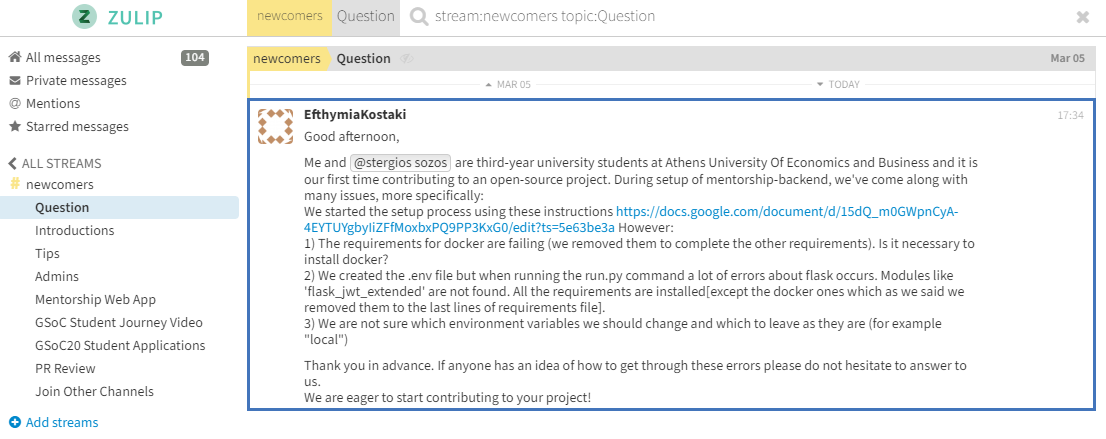
\includegraphics[totalheight=8cm, width=18cm]{Setup-problems.png}}
    \caption{Setup Problems}
    \label{fig:verticalcell}
\end{figure}
%-----

After a vary insightful discussion with the community we were able to build the project and also share our insights in how we solved these problems if a new contributor wants to set up this project!
% Image
\begin{figure}[tph!]
\centerline{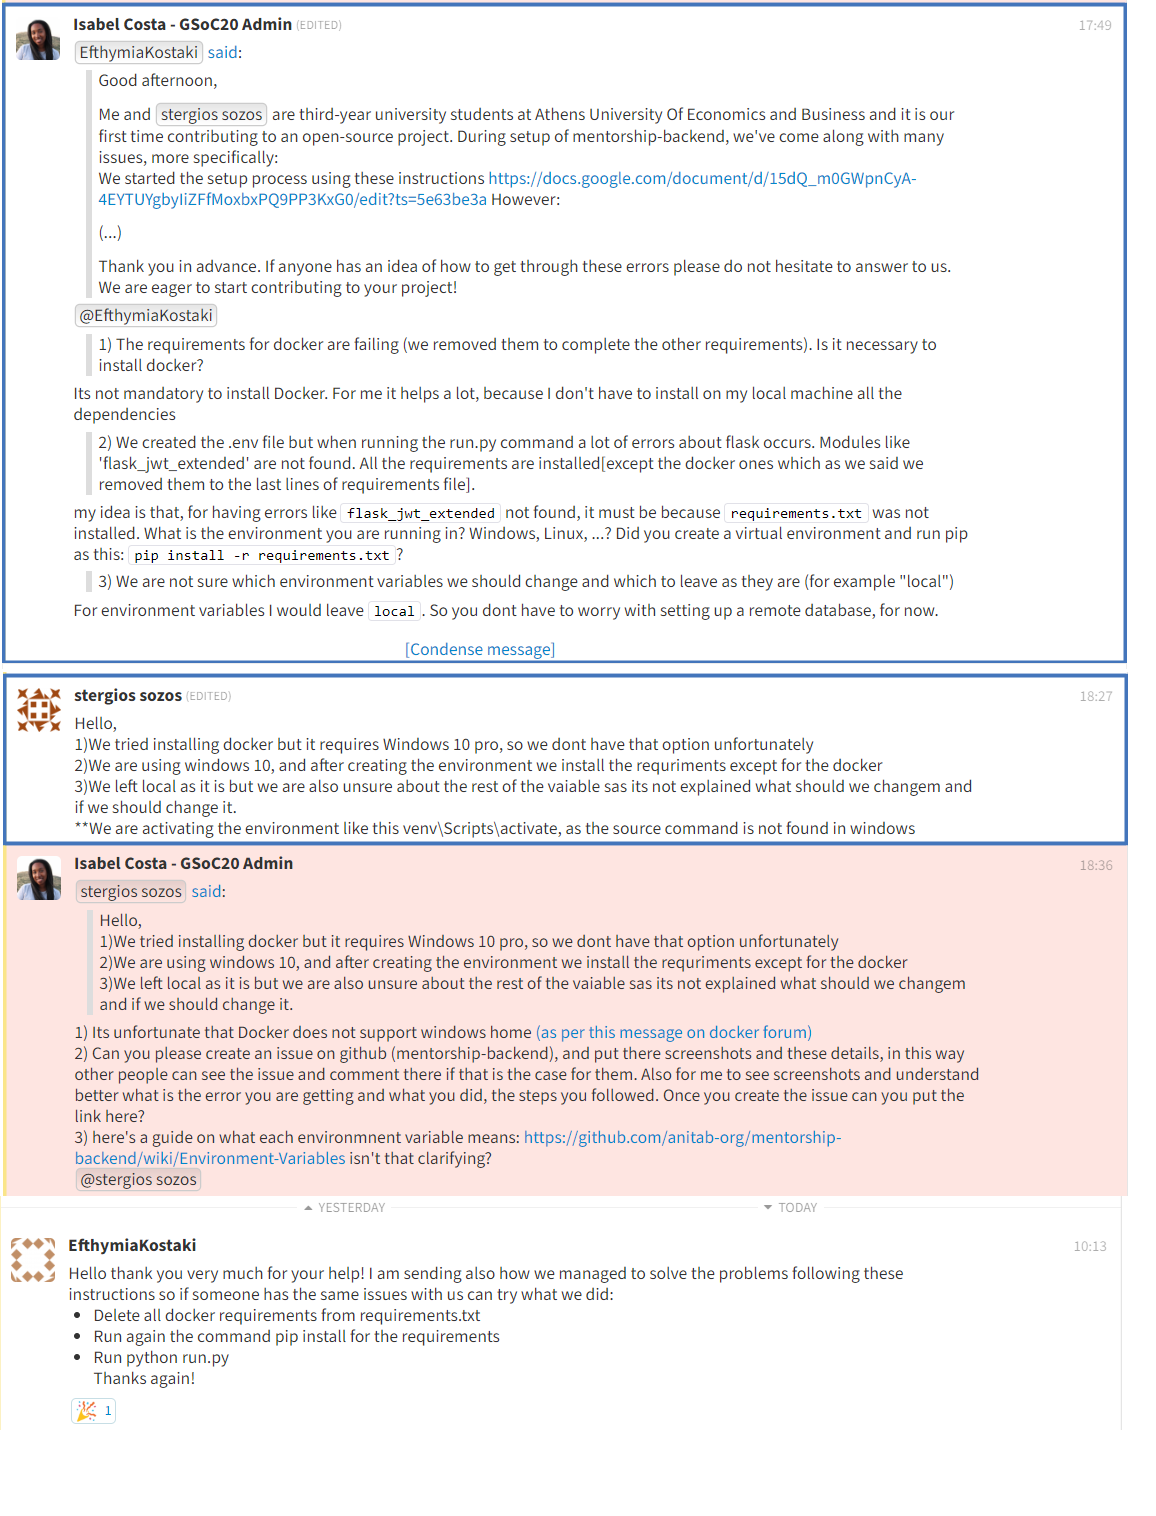
\includegraphics[totalheight=16cm, width=16cm]{Setup-discussion.png}}
    \caption{Setup Discussion}
    \label{fig:verticalcell}
\end{figure}
%-----

\vfill
\clearpage

\section{Mentorship Backend}

\hspace{0.5cm}Mentorship System is an application that matches women in tech to mentor each other, on career development, through 1:1 relations during a certain period of time. The project is deplyed in Heroku in this link: https://mentorship-backend-temp.herokuapp.com/. The backend is based on a REST API. There is also the Android client of the app for creating the interface for the users. [3]

The repository has the following permanent branches:
\begin{itemize}
 \item \textbf{master}: This contains the code which has been released.
 \item \textbf{develop}: This contains the latest code. All the contributing PRs must be sent to this branch. When we want to release the next version of the app, this branch is merged into the master branch. 
\end{itemize}

\section{Initial Communication with the community}
% Image
\begin{figure}[tph!]
\centerline{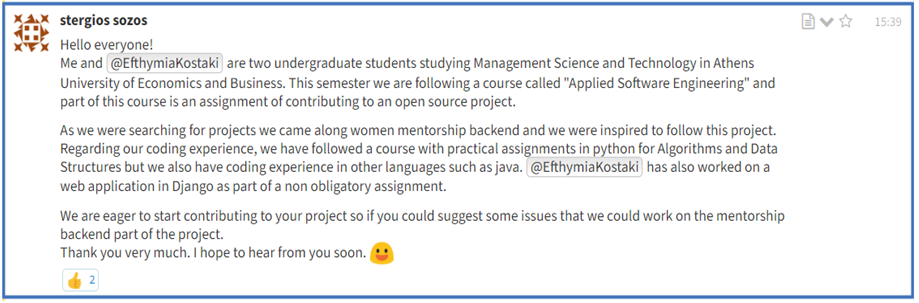
\includegraphics[totalheight=5cm]{FirstCommunication.png}}
    \caption{First Communication}
    \label{fig:verticalcell}
\end{figure}
%-----
\vfill
\clearpage

\section{Our contribution}
Here is a full list of the parts of our contribution in a wide range of aspects such as quality assurance, user interface, code and testing. 

\subsection{Issue 1 - Create Quality Assurance table for Update Task API - \emph{Merged} \#473}

\subsubsection{Issue}
% Image
\begin{figure}[tph!]
\centerline{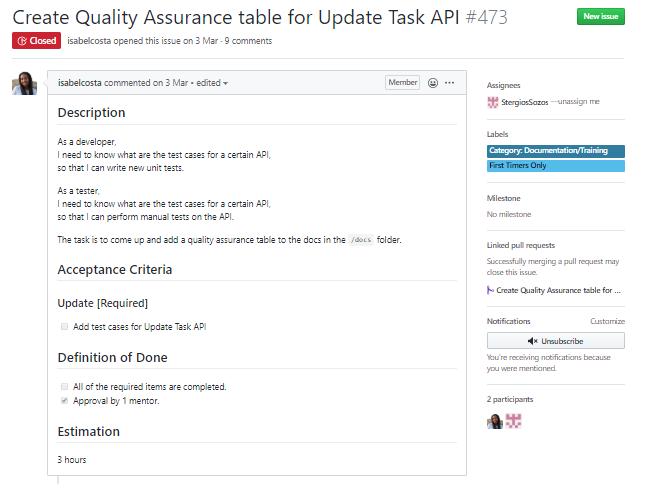
\includegraphics[totalheight=13cm, width=15cm]{issue473.png}}
    \caption{Issue 473}
    \label{fig:verticalcell}
\end{figure}
%-----

\vfill
\clearpage

\subsubsection{Communication with the team}

\hspace{0.5cm}This issue was labeled for first-time contributors so we asked if we could work on this issue to understand the project better. The main maintainer was really helpful and answering out questions soon after we sent them.
Fisrtly, we thought that new unit tests were required, combined with the quallity assurane table, but after our comminucation it was clear to us that only the table had to be completed, as the tests already existed.
While doing this table, by executing some tasks, we found out that there was a possible problem, and an issue had to be raised, as the maintainer agreed.
\subsubsection{Documentation}
This issue was labeled , among other labels, as documentation, for improvmenets or additions to documentation.
\subsubsection{Our work}
\hspace{0.5cm}We worked in the default develop branch for this issue. We came to realize that this was a wrong startegy so in all other issues we created a specific branch for them. We tried to write meaningful messages in our commit messages always following the commit style guide suggested by the project. When we thought that the commit message was not understandable enough we wrote a body in our commit messages and documented further our change.

Regarding the way we created the table, firstly we found th file that we had to change, which was easy as the creator of the issue had already mentioned which one is it. Then the difficult part was understanding what exaclty we had to write on the table and how to test it. After going through the test cases to take some ideas on what we could test on the backend server, we tried to create an account on the server. We used temp mail, as it was suggested, and created 4 profiles, so we could test all the possibilities we wanted. For example, we needed a user with a non-verified email, and one with verified. 
Then, we strugled a lot to find out the parameters-arguments that were needed for completing the task we wanted. For example a "token" was required but there was nowhere any explanation about this token. After some searching, we realised that when a user is logging in the server, the success message also provides this token. But even the way that we needed to insert the token was unusual, as we had to write "Bearer <token here>"
Finally, when we had our users ready, and new how to use the backend server, we finallly tested all the scenarios and write them down in the table.

\subsubsection{Testing}
\hspace{0.5cm}Since this change was a change in the UI we did not need to run local testing or write new tests. Instead, our changes were visible in github, as the file was written in markdown language and that's how we verified that our changes were visible and correct. Also, we verified that the continuous integration testing in Travis CI was passing. 
\subsubsection{Code Reviews}
\hspace{0.5cm}Our pull request received immidiate feedback and reviews. our first PR needed some important changes:
1) We were checking multiple failing variables, but only one was required each time. For example we were testing the result of the task with arg1 and arg2 causing the task to fail but arg1 was enough and a separate test for arg2 was required. 
2) We were describing a variable/argument as "wrong" but we did not specify why it was wrong. For example, a user could not exist, or he could have not accepted the terms, or even not verufy his email address. These 3 cases should be separate and specified.
3) We reffered the users with pronouns and we had to make it general ("the user" instead of "he").
4) We had to fix merge conflocts as the PR was approved later.
 Also, other contributors viewed our changes and accepted them. 
\subsubsection{Change}
% Image
\begin{figure}[tph!]
\centerline{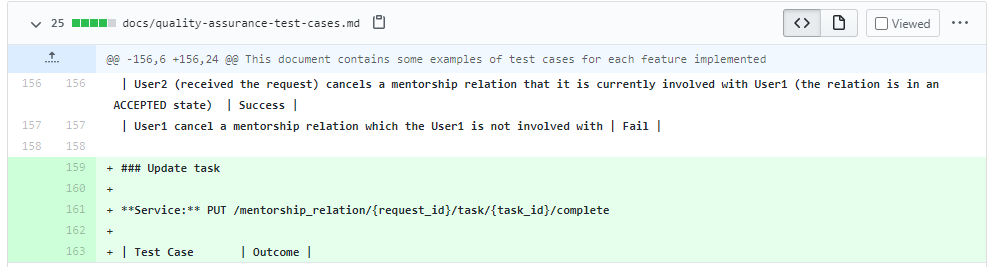
\includegraphics[totalheight=13cm, width=15cm]{517Changes_1.png}}
    \caption{Files changed on 517}
    \label{fig:verticalcell}
\end{figure}
%-----
% Image
\begin{figure}[tph!]
\centerline{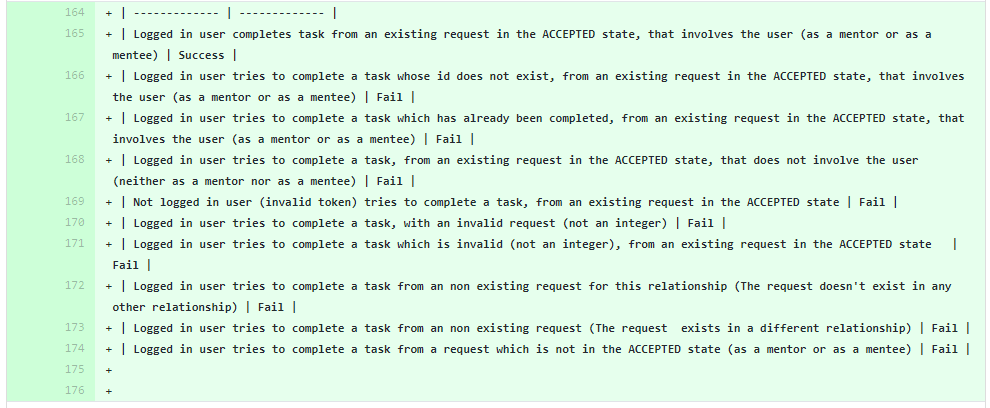
\includegraphics[totalheight=13cm, width=15cm]{517Changes_2.png}}
    \caption{Files changed on 517}
    \label{fig:verticalcell}
\end{figure}
%-----
\vfill
\clearpage
\subsection{Issue 2 -Fix description messages on Mentorship Relation - \emph{Merged} \#554}
\subsubsection{Issue}
% Image
\begin{figure}[tph!]
\centerline{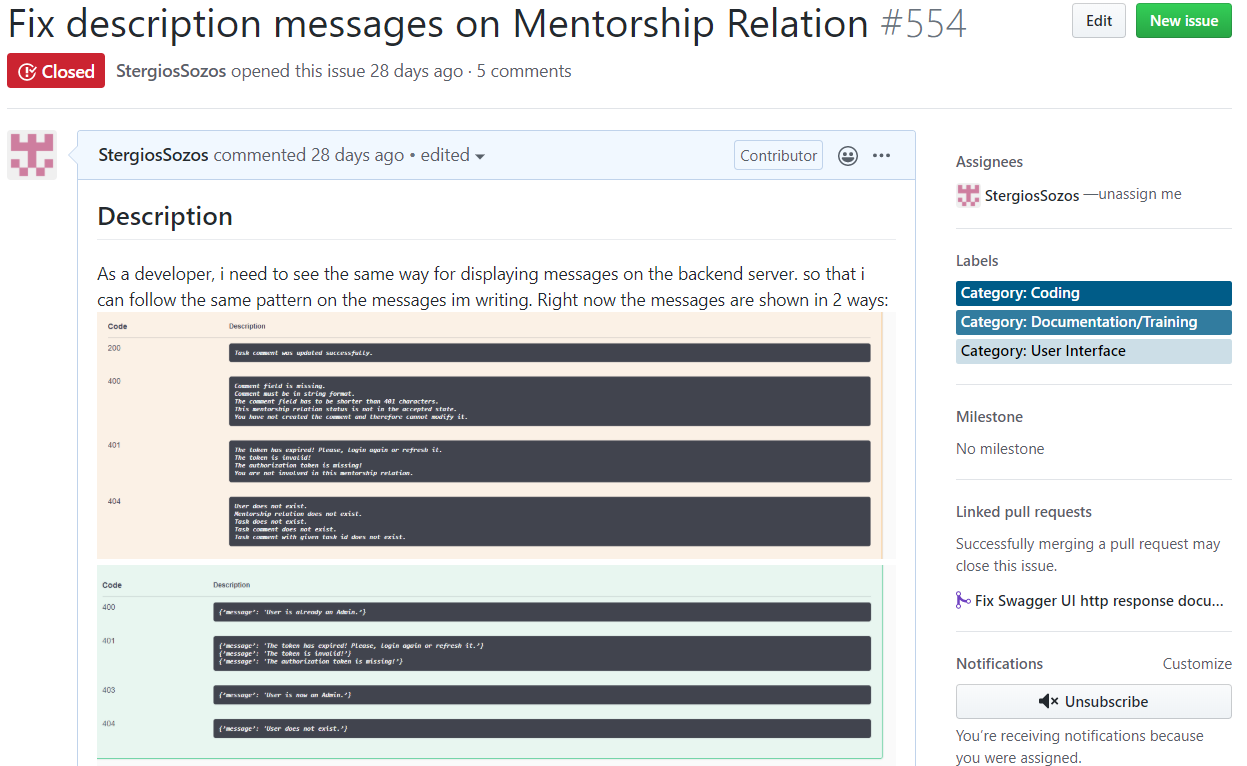
\includegraphics[totalheight=13cm, width=16cm]{issue554part1.png}}
    \caption{Issue 554-1}
    \label{fig:verticalcell}
\end{figure}
%-----

\vfill
\clearpage

\subsubsection{Communication with the team}
After finding out the problem on the backend server, we created the issue, but we did not know which style of the two we found was the correct one. Thus we posted also in zulip, in the corresponding channel, where we were also posting questions we had when we were working on other issues. The maintainer saw our post and found our observation very interesting and imoprtant -she also mentioned that on the merge of the branch, and congratsed us for pointing out the mistake and for sloving it. Therefore, after clearing out which style was the correct one, she assigned us to the issue.
\subsubsection{Documentation}
This issue was labeled, among other labels, as documentation, for improvmenets or additions to documentation.
\subsubsection{Our work}
After studing f-strings and how they work, we went through the code that is responsible for showing the description on the backend. We tracked the file, and the part that needed change, and we realised that dictionaries were used in a wrong way. Instead of printing the whole dictionary, for example messages.TASK\_COMMENT\_WAS\_DELETED\_SUCCESSFULLY, only the word of the key-"message" was printed, for example messages.TASK\_COMMENT\_WAS\_DELETED\_SUCCESSFULLY["message"]. Thus, we removed the specific key, and then the whole dictionary was showed, as was requested by the maintainer. We also used f-strings, in cases were the correct message appeared but without the use of f-strings, which was in the code standards of the project.
\subsubsection{Testing}
\begin{itemize}
\item While running the local server and checking the UI the changes are visible.
\item All Travis CI tests have passed
\end{itemize}
\subsubsection{Code Reviews}
There were not any changes requested for our PR. Some tests were asked, to other reviewers for checking if our changes were visible after merging this branch, which was confirmed by other reviewers, and our PR was accepeted and merged.
\subsubsection{Change}
% Image
\begin{figure}[tph!]
\centerline{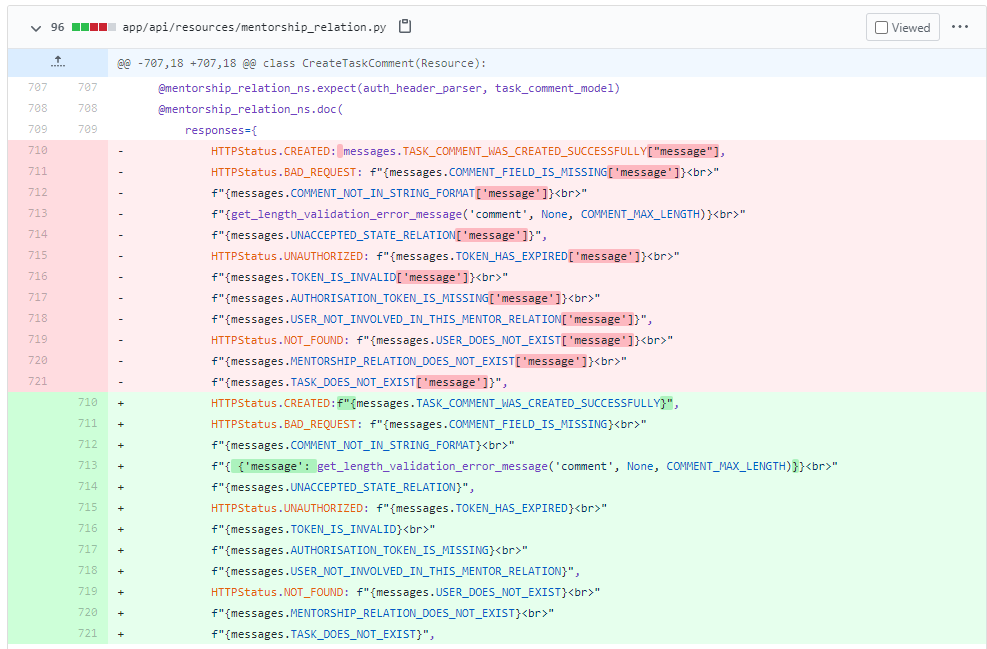
\includegraphics[totalheight=15cm, width=16cm]{567Changes_1.png}}
    \caption{Issue 567\_change1}
    \label{fig:verticalcell}
\end{figure}
%-----

% Image
\begin{figure}[tph!]
\centerline{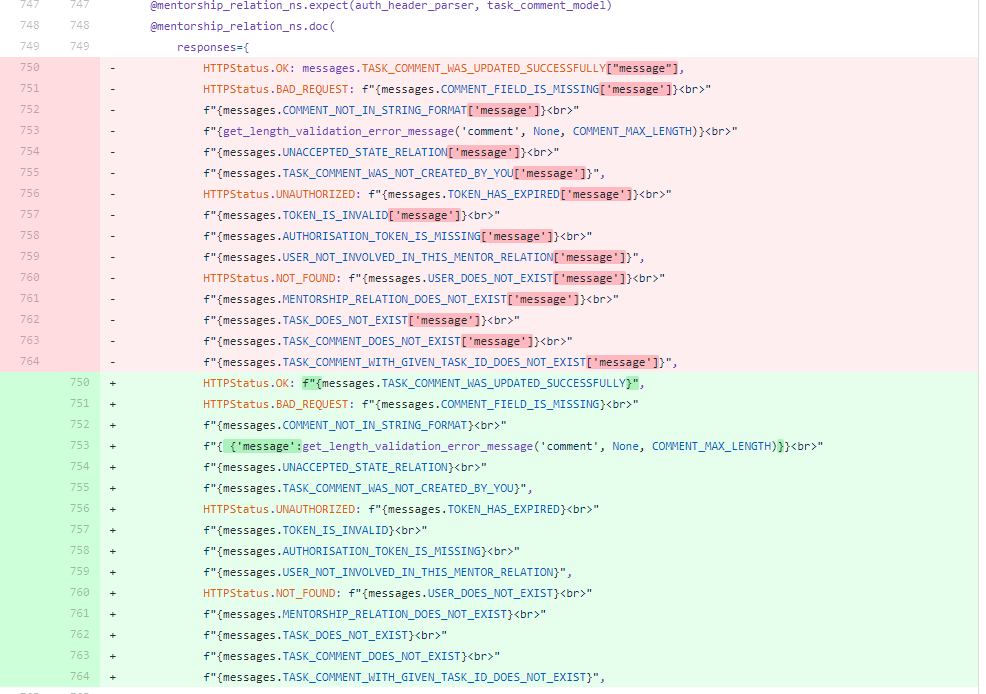
\includegraphics[totalheight=15cm, width=16cm]{567Changes_2.png}}
    \caption{Issue 567\_change2}
    \label{fig:verticalcell}
\end{figure}
%-----
% Image
\begin{figure}[tph!]
\centerline{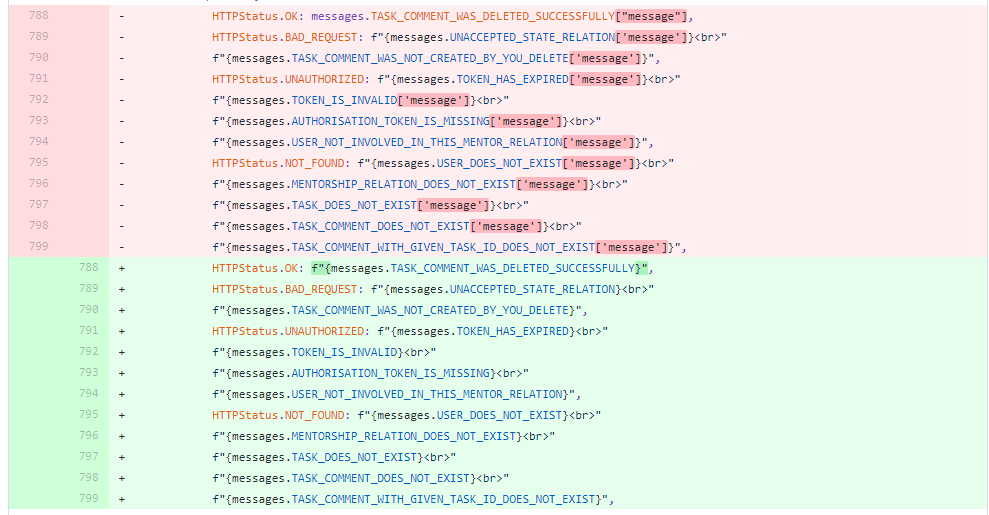
\includegraphics[totalheight=15cm, width=16cm]{567Changes_3.png}}
    \caption{Issue 567\_change3}
    \label{fig:verticalcell}
\end{figure}
%-----
% Image
\begin{figure}[tph!]
\centerline{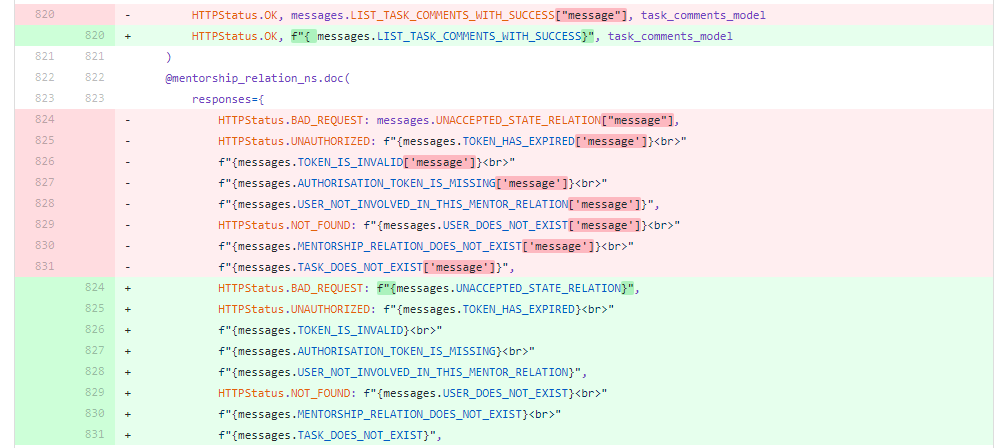
\includegraphics[totalheight=15cm, width=16cm]{567Changes_4.png}}
    \caption{Issue 567\_change4}
    \label{fig:verticalcell}
\end{figure}
%-----

\vfill
\clearpage
\subsection{Issue 3 - `Complete task` not including all the necessary information when request id is not in accepted mode - \emph{Accepted} \#537}

\subsubsection{Issue}
% Image
\begin{figure}[tph!]
\centerline{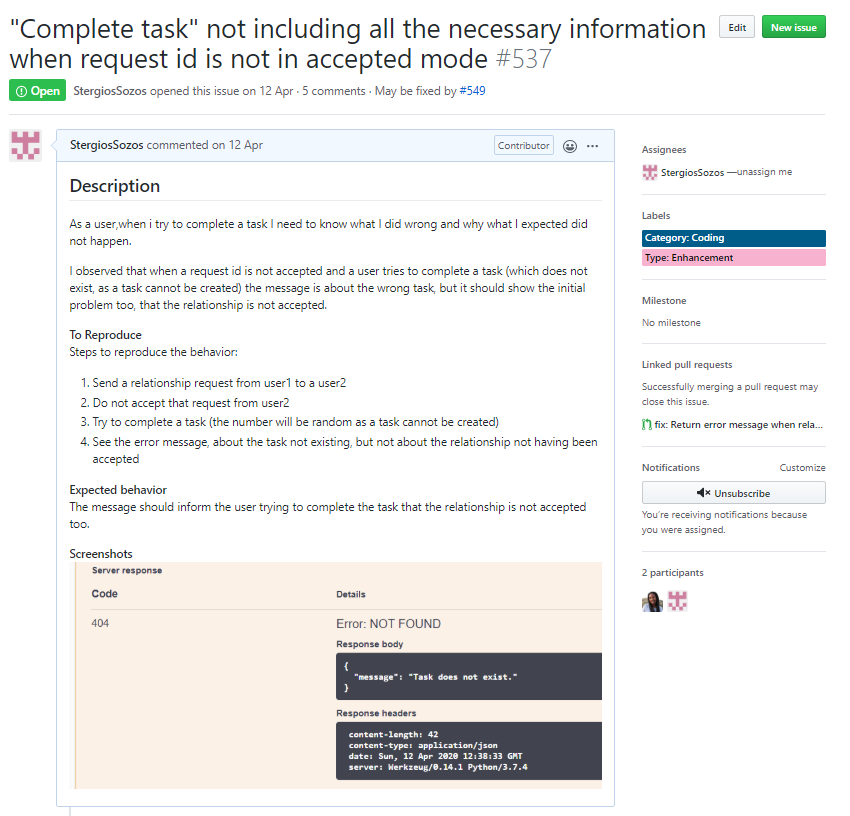
\includegraphics[totalheight=15cm, width=16cm]{issue537.png}}
    \caption{Issue 537}
    \label{fig:verticalcell}
\end{figure}
%-----

\vfill
\clearpage
\subsubsection{Communication with the team}
We had already talked about this issue with the maintainer in a PR, so after the maintainer's approval, we opened a new issue, and got assigned to it. We also clarified, that the solution suggested on this issue, is giving higher priority to a specific argument, whih was the state of the relationship status, instead of the one that was then highest, which was the existence of the task.

\subsubsection{Our work}

We added an if statement before the existings one, so that it will be prioratized, and included the new possible responses on the responses board on the backend server. After that we changed the hardcoded status (i.e. 400,401 etc) to http status. Then, we changed the way messages were printed into f strings and added some blank spaces that were needed. Finally, we wrote a unit test for the added if statement.

After the original 
\subsubsection{Testing}
Initially, we didn't have any unit testing for the speific change, and we tested it only on the backend server, and we also confirmed that the continuous integration testing in Travis CI was passing. 
After our PR was reviewed and after all the changes requested had been done, an additional test was asked, a unit test. To create this, we needed to also add a user to the database and create a new relation of this user with another user.

\subsubsection{Code Reviews}
The main part of the PR was approved, and only some minor changes were asked, regarding new standards(http status instead of harcoded numbers, f strings for printing messages) and a blank line to separate visually validation sections. After these minor changes, a unit test was asked.
\subsubsection{Change}
% Image
\begin{figure}[tph!]
\centerline{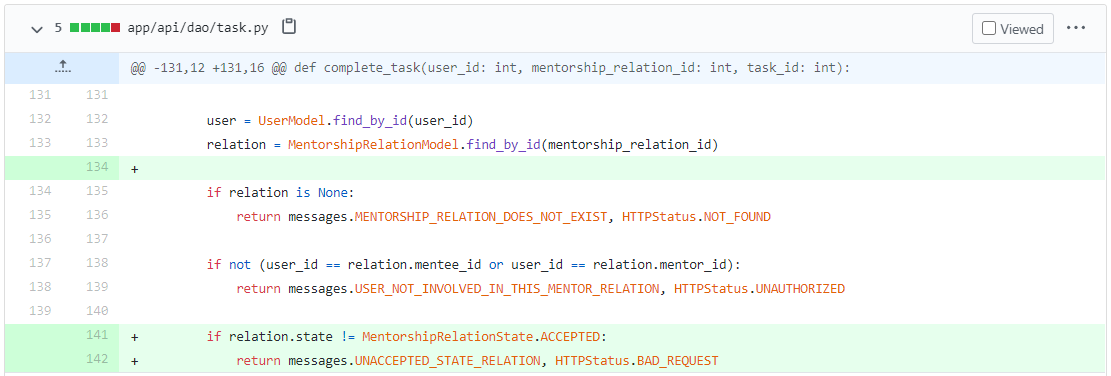
\includegraphics[totalheight=15cm, width=16cm]{549Changes_dao_task.png}}
    \caption{549Changes\_dao\_task}
    \label{fig:verticalcell}
\end{figure}
%-----
% Image
\begin{figure}[tph!]
\centerline{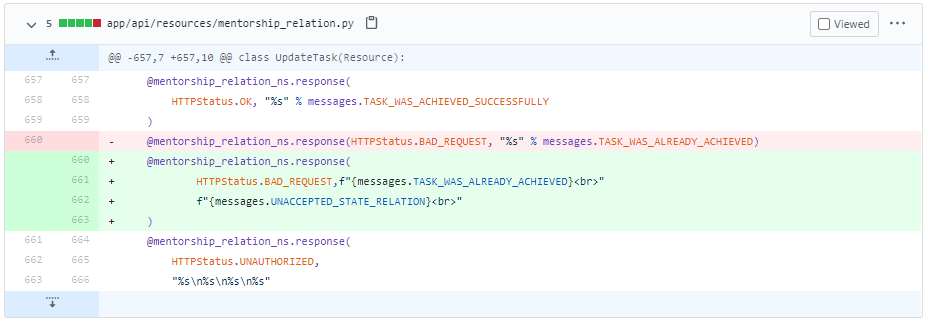
\includegraphics[totalheight=15cm, width=16cm]{549Changes_mentorship_relation.png}}
    \caption{549Changes\_mentorship\_relation}
    \label{fig:verticalcell}
\end{figure}
%-----
% Image
\begin{figure}[tph!]
\centerline{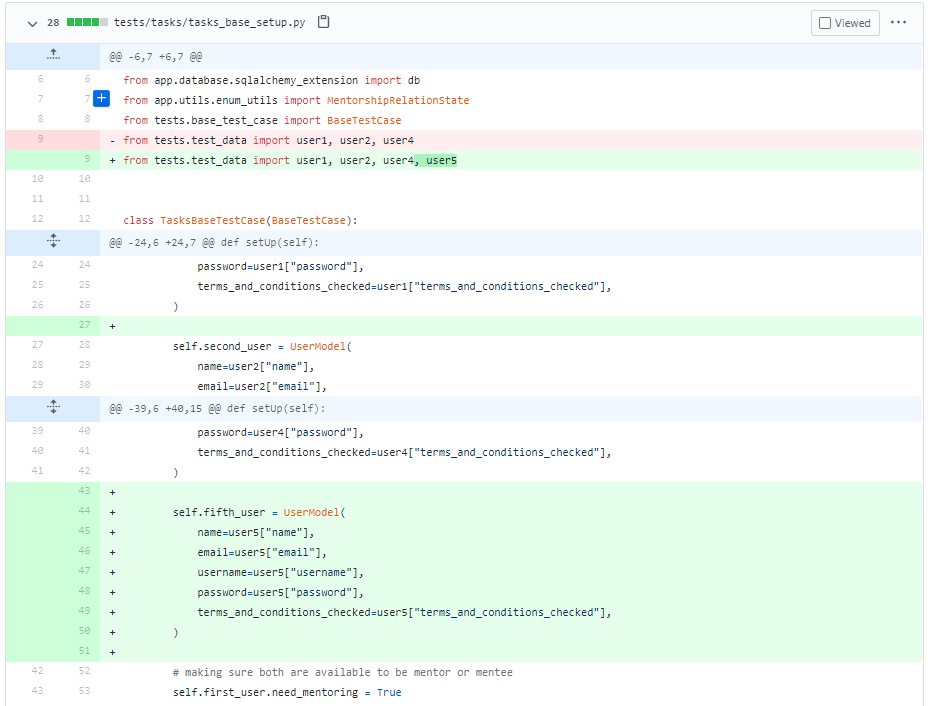
\includegraphics[totalheight=15cm, width=16cm]{549Changes_tasks_base_setup.png}}
    \caption{549Changes\_tasks\_base\_setup}
    \label{fig:verticalcell}
\end{figure}
%-----
% Image
\begin{figure}[tph!]
\centerline{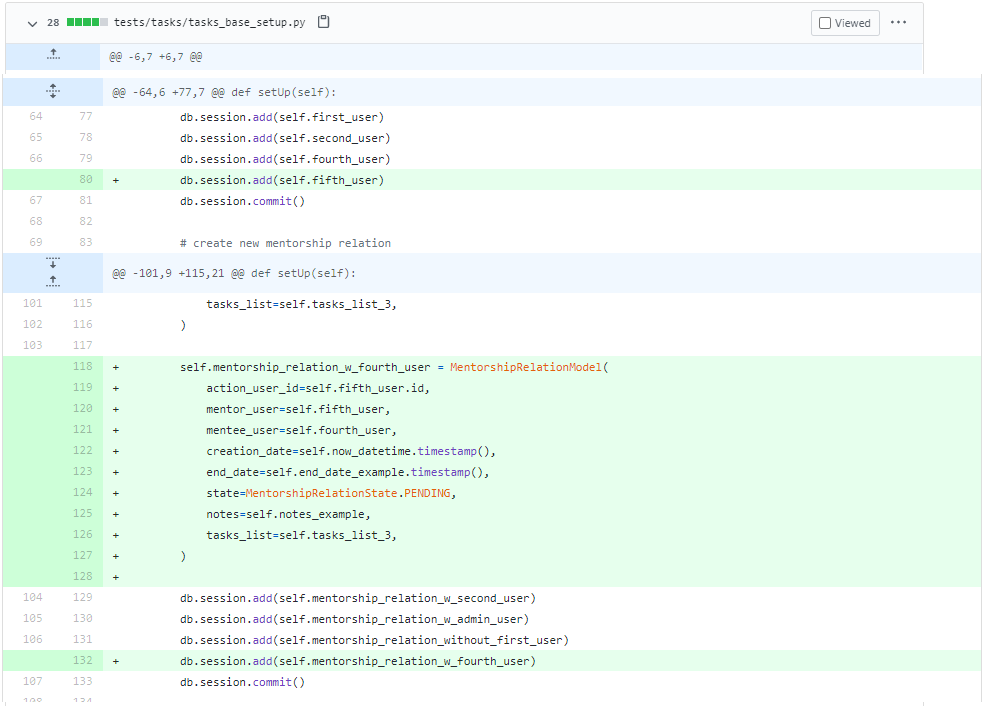
\includegraphics[totalheight=15cm, width=16cm]{549Changes_tasks_base_setup_2.png}}
    \caption{549Changes\_tasks\_base\_setup\_2}
    \label{fig:verticalcell}
\end{figure}
%-----
% Image
\begin{figure}[tph!]
\centerline{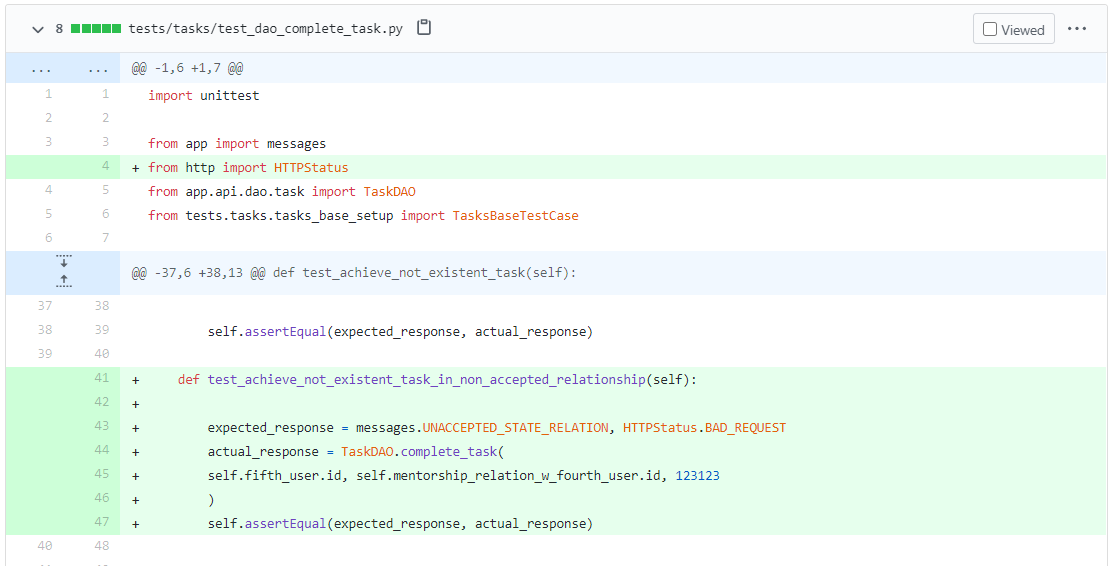
\includegraphics[totalheight=15cm, width=16cm]{549Changes_test_dao_complete_task.png}}
    \caption{549Changes\_test\_dao\_complete\_task}
    \label{fig:verticalcell}
\end{figure}
%-----
% Image
\begin{figure}[tph!]
\centerline{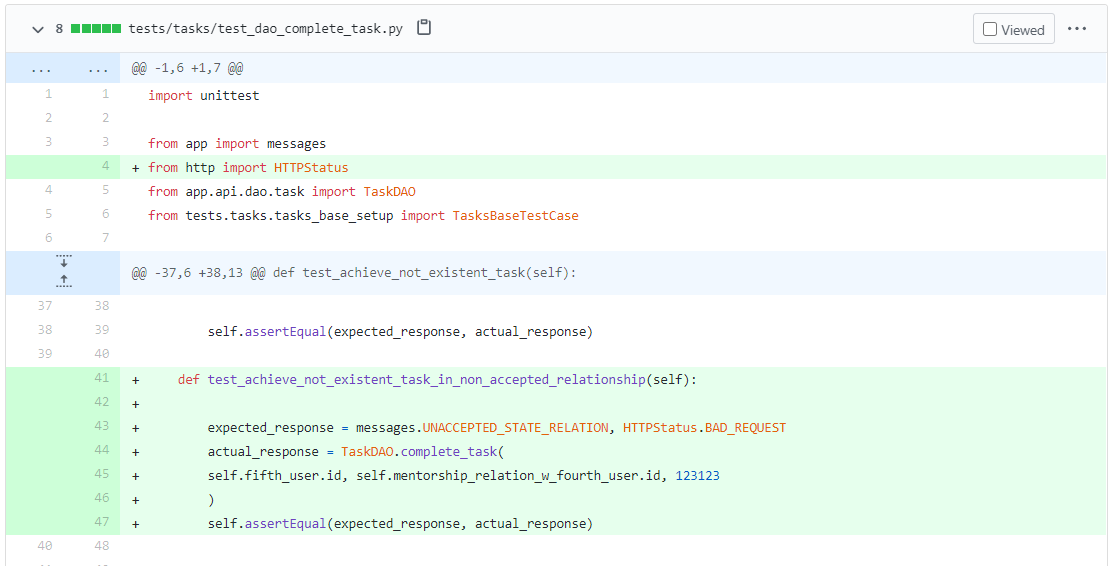
\includegraphics[totalheight=15cm, width=16cm]{549Changes_test_dao_complete_task.png}}
    \caption{549Changes\_test\_dao\_complete\_task}
    \label{fig:verticalcell}
\end{figure}
%-----
% Image
\begin{figure}[tph!]
\centerline{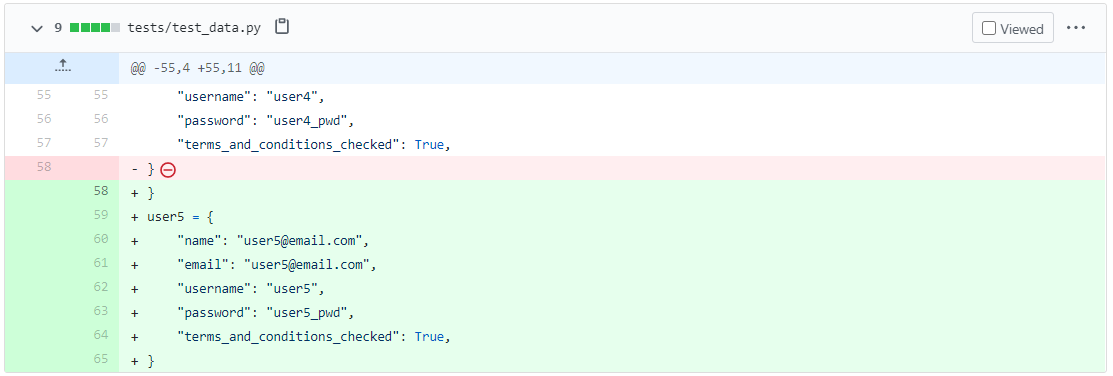
\includegraphics[totalheight=15cm, width=16cm]{549Changes_test_data.png}}
    \caption{549Changes\_test\_data}
    \label{fig:verticalcell}
\end{figure}
%-----
\vfill
\clearpage

\subsection{Issue 4 - Improve the description of the app on the Swagger UI docs - \emph{Merged} \#482}
\subsubsection{Issue}
\hspace{0.5cm}This issue was referring to the description of the app which the developers view if they have cloned the repository locally or in the deployed app remotely in Heroku.
% Image
\begin{figure}[tph!]
\centerline{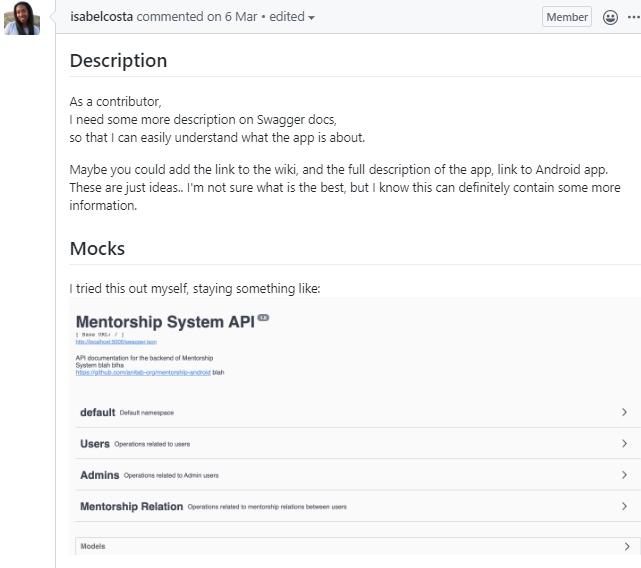
\includegraphics[totalheight=12cm, width=14cm]{issue482.png}}
    \caption{Issue 482}
    \label{fig:verticalcell}
\end{figure}
%-----

\vfill
\clearpage
\subsubsection{Communication with the team}										
\hspace{0.5cm}This issue was labeled for first-time contributors so we asked if we could work on this issue to understand the project better. The main maintainer was really helpful and answering out questions soon after we sent them. We realized while working on the issue that there was an issue with the namespaces since there was a default namespace which was not referring to any API. We decided to ask about this if this was intentional or it was a problem in the UI. In figure shown above this problem is visible in the `default namespace` resource. Isabel (the main mainteiner and creator of the project) told us that this was really an issue and that she did not know how to solve it. She suggested that if we solve this problem we can commit the change in the current pull request so as to further expand it so it includes the solution of this problem as well.

\subsubsection{Our work}

\hspace{0.5cm}We worked in the default develop branch for this issue. We came to realize that this was a wrong startegy so in all other issues we created a specific branch for them. We tried to write meaningful messages in our commit messages always following the commit style guide suggested by the project. When we thought that the commit message was not understandable enough we wrote a body in our commit messages and documented further our change.

Regarding the initial issue, it turned out to be hard for us t understand which part on the project we should change in order for our changes to be visible in the User Interface. We used Atom, the text editor, to find the parts of the software which had the initial description we wanted to change. They were two, the swagger.json and the api\_extension.py file. Since we did not know which was the correct file we should change we decided to change both of them. The correct one turned out to be the api\_extension.py file. We were able to view our changes locally.

Regarding the new part of the issue we identified and proposed, we needed to understand were the problem was coming from. It could have been from the call inside the specific resources or in some other part of the project. We searched a lot and found the documentation of the flask\_restplus library which was used in the file we wanted to change. We found the method Api() and which parameters it could include and we were able to change the arguments and change the name of the `default namespace'. The documentation however, did not help us fix the actual issue which was to remove this resource. We searched again and found out that this library was actually open-source. In the issues of the Github repository we were able to find an issue about the same problem we had and a suggested solution to it. By implementing this code we were able to solve the issue.
\subsubsection{Testing}
\hspace{0.5cm}Since this change was a change in the UI we did not need to run local testing or write new tests. Instead, our changes were visible in the localhost in our browser and that's how we verified that our changes were visible and correct. Also, we verified that the continuous integration testing in Travis CI was passing. 
\subsubsection{Code Reviews}
\hspace{0.5cm}Our pull request received immidiate feedback and reviews. Since the change was in the User Interface, Isabel asked us to include a screenshot of the change proposed in the description. Also, other contributors viewed our changes and accepted them. 
\subsubsection{Change}
\hspace{0.5cm}The merged change is this:
% Image
\begin{figure}[tph!]
\centerline{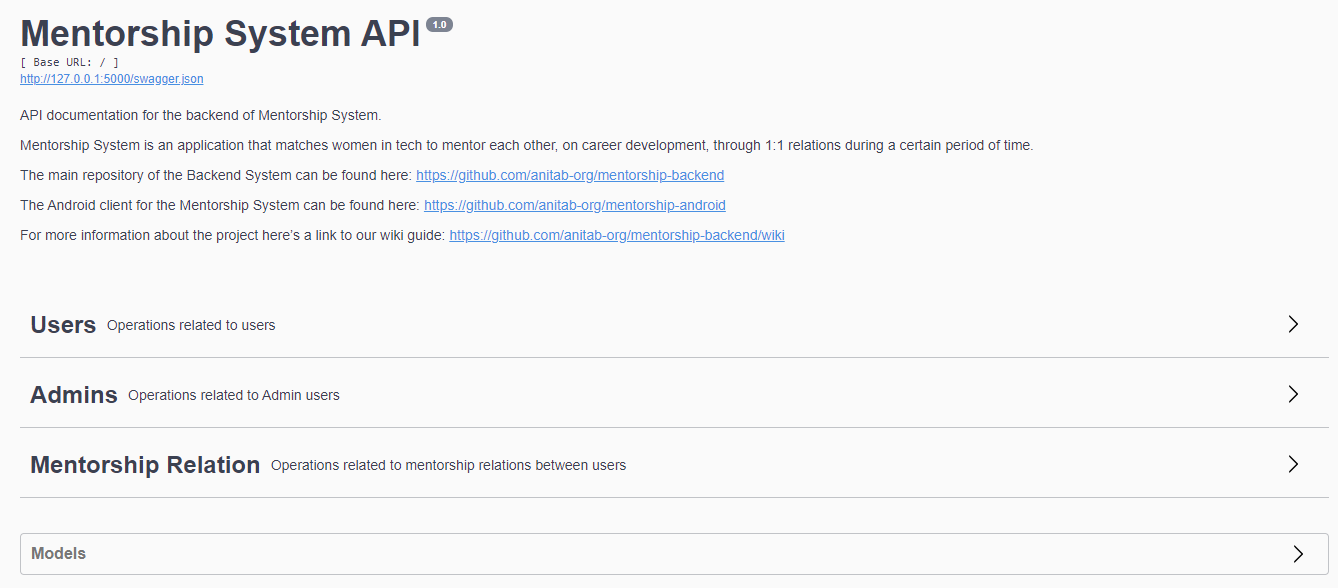
\includegraphics[totalheight=8cm, width=18cm]{issue482-UI.png}}
    \caption{Change in the UI}
    \label{fig:verticalcell}
\end{figure}
\vfill
\clearpage
%-----
\hspace{0.5cm}This change required to change these files and add new code:
% Image
\begin{figure}[tph!]
\centerline{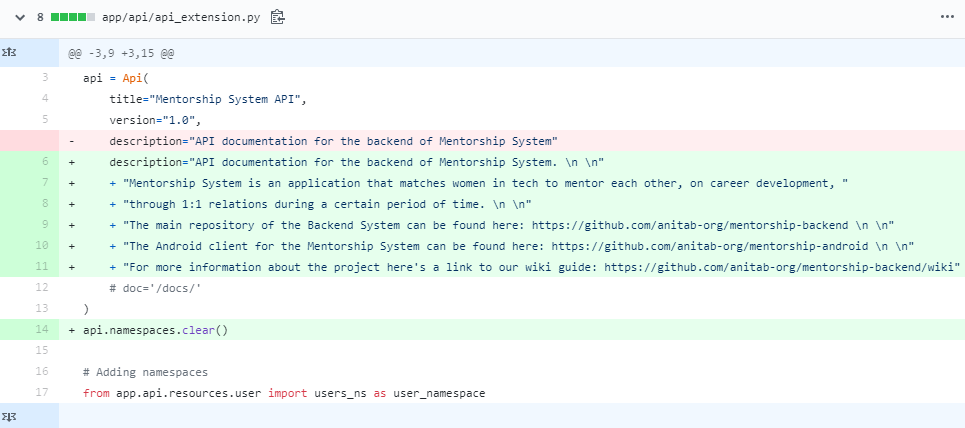
\includegraphics[totalheight=8cm, width=18cm]{change-issue482.png}}
    \caption{Code change}
    \label{fig:verticalcell}
\end{figure}
%-----

\vfill
\clearpage
\subsubsection{Happy Moments!}
The creator and main maintainer of the project congratulated us for our effiort and change in the UI which urged us to find other aspects of the software in which we could contribute.
% Image
\begin{figure}[tph!]
\centerline{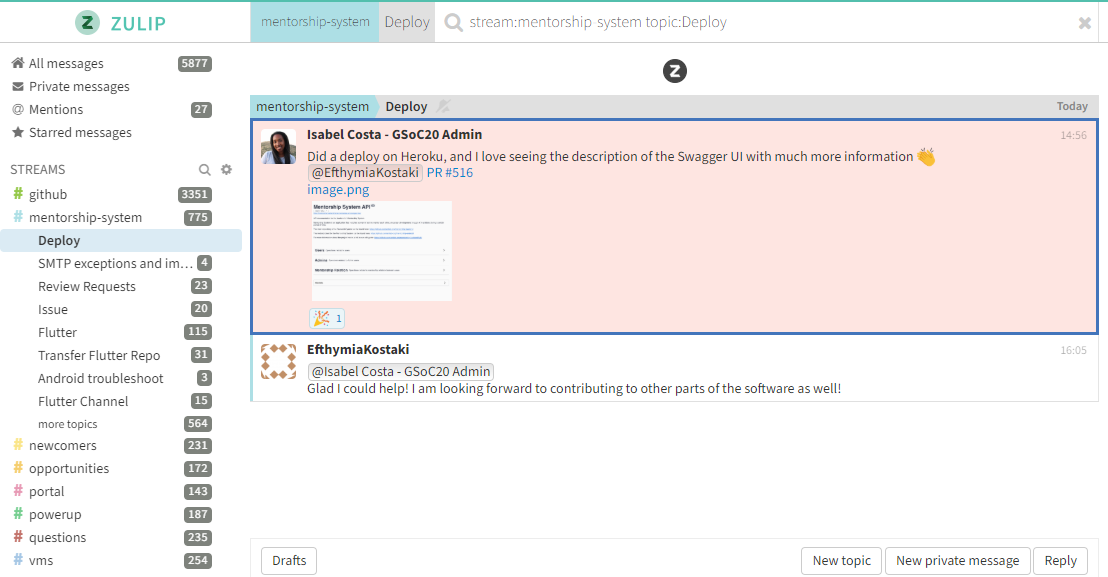
\includegraphics[totalheight=10cm, width=15cm]{Happy-Moments.png}}
    \caption{Happy Moments!}
    \label{fig:verticalcell}
\end{figure}
%-----
\vfill
\clearpage

\subsection{Issue 5 - Optimise code for repeated code in `app/api/dao/user.py` `get\_user\_dashboard`- \emph{Accepted} \#418}
\subsubsection{Issue}
\hspace{0.5cm}This issue required simplifying a method which was around 200 lines in to less.We successfully removed 70 lines with repeated code.
% Image
\begin{figure}[tph!]
\centerline{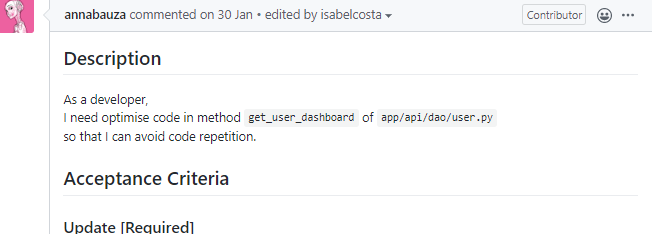
\includegraphics[totalheight=5cm, width=14cm]{issue418.png}}
    \caption{Issue 418}
    \label{fig:verticalcell}
\end{figure}
%-----
\vfill
\clearpage
\subsubsection{Communication with the team}
\hspace{0.5cm}It was crucial for us to understand how we could verify that our changes were correct and that the project was having the same functionality as before. So we asked in the issue how we could verify that or if it was necessary to write some new unit tests. The maintainer told us that we should just verify that the unit tests are working as before.

\subsubsection{Our work}
\hspace{0.5cm}We created a specific branch for this issue first locally and then add this branch to our remote repository. We tried to write meaningful messages in our commit messages always following the commit style guide suggested by the project. When we thought that the commit message was not understandable enough we wrote a body in our commit messages and documented further our change.

Firstly, we realized that the as\_mentor and as\_mentee dictionaries were exactly the same and that we could delete the initialization of one and copy it to the other one. Since, these dictionaries had also subdictionaries we found out we should not copy them using the traditional copy() method since in some occasions when changing the subdictionary in the one dictionary could actually change the other one as well. To solve this problem, we found out the copy library which offers a method named deepcopy() which could solve our problem. We used this method and successfully deleted 15 lines of repeated code.

The second part of our work was to create a method which could remove further the repeated code. All the dictionary was assesed this way for more than 100 lines:
\lstset{language=Python}
\begin{lstlisting}
as_mentee["received"]["completed"] = [
    relation.response
   for relation in mentee_received_relations
   if relation.state == MentorshipRelationState.COMPLETED
]
as_mentee["received"]["cancelled"] = [
   relation.uuresponse
   for relation in mentee_received_relations
   if relation.state == MentorshipRelationState.CANCELLED
]
\end{lstlisting}

After we understood which was the problem we tried to experiment and decide which parameters should this method have. We decided that these two were enough. First, the mentor\_or\_mentee\_received\_or\_sent which would include the relations of the mentee or the mentor and if these relations are received or sent and the mentorship\_relation\_state\_wanted which could take one of these values:
\begin{itemize}
  \item PENDING
  \item CANCELLED
  \item COMPLETED
  \item REJECTED
\end{itemize}

\hspace{0.5cm}This method is static as they are all the other methods in this file and has a for loop similar to the initial one taking use of all the arguments and returns a list to be added in each subdictionary.
\subsubsection{Testing}
\hspace{0.5cm}Since the maintainer told us that we do not need to write unit tests about our change we verified that all the local testing was passing and of course that the continuous integration testing in Travis CI was passing.
\subsubsection{Code Reviews}
\hspace{0.5cm}Unfortunately, this pull request has not been reviewed yet but we asked the main maintainer to do that as soon as possible. She said that she does not have much bandwidth and will try get back to us in that as soon as possible.

% Image
\begin{figure}[tph!]
\centerline{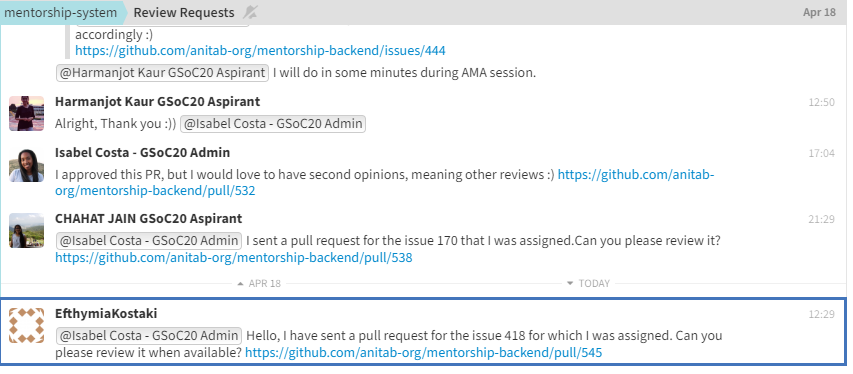
\includegraphics[totalheight=7cm, width=15cm]{issue418-ask-for-review.png}}
    \caption{Issue 418 - Ask for review}
    \label{fig:verticalcell}
\end{figure}
%-----
\vfill
\clearpage

\subsubsection{Change}
\hspace{0.5cm}Our proposed change is this:
\lstset{language=Python}
\begin{lstlisting}
@staticmethod
def get_state(mentor_or_mentee_received_or_sent, 
                       mentorship_relation_state_wanted):
   value = [relation.response
   for relation in mentor_or_mentee_received_or_sent
   if relation.state == mentorship_relation_state_wanted]
   return value
\end{lstlisting}
\lstset{language=Python}
\begin{lstlisting}
as_mentor = copy.deepcopy(as_mentee)
as_mentee["received"]["accepted"] = 
             UserDAO.get_state(mentee_received_relations, 
             MentorshipRelationState.ACCEPTED)
as_mentee["received"]["rejected"] = 
             UserDAO.get_state(mentee_received_relations, 
             MentorshipRelationState.REJECTED)
as_mentee["received"]["completed"] = 
             UserDAO.get_state(mentee_received_relations, 
             MentorshipRelationState.COMPLETED)
as_mentee["received"]["cancelled"] = 
             UserDAO.get_state(mentee_received_relations, 
             MentorshipRelationState.CANCELLED)
as_mentee["received"]["pending"] = 
            UserDAO.get_state(mentee_received_relations, 
            MentorshipRelationState.PENDING)
as_mentor["received"]["accepted"] = 
            UserDAO.get_state(mentor_received_relations, 
            MentorshipRelationState.ACCEPTED)
as_mentor["received"]["rejected"] = 
            UserDAO.get_state(mentor_received_relations, 
            MentorshipRelationState.REJECTED)
as_mentor["received"]["completed"] = 
            UserDAO.get_state(mentor_received_relations, 
            MentorshipRelationState.COMPLETED)
as_mentor["received"]["cancelled"] = 
            UserDAO.get_state(mentor_received_relations, 
            MentorshipRelationState.CANCELLED)
as_mentor["received"]["pending"] = 
            UserDAO.get_state(mentor_received_relations, 
            MentorshipRelationState.PENDING)
as_mentee["sent"]["accepted"] =
            UserDAO.get_state(mentee_sent_relations, 
            MentorshipRelationState.ACCEPTED)
as_mentee["sent"]["rejected"] = 
            UserDAO.get_state(mentee_sent_relations, 
            MentorshipRelationState.REJECTED)
as_mentee["sent"]["completed"] = 
            UserDAO.get_state(mentee_sent_relations, 
            MentorshipRelationState.COMPLETED)
as_mentee["sent"]["cancelled"] = 
            UserDAO.get_state(mentee_sent_relations, 
            MentorshipRelationState.CANCELLED)
as_mentee["sent"]["pending"] = 
            UserDAO.get_state(mentee_sent_relations, 
            MentorshipRelationState.PENDING)
as_mentor["sent"]["accepted"] = 
            UserDAO.get_state(mentor_sent_relations, 
            MentorshipRelationState.ACCEPTED)
as_mentor["sent"]["rejected"] = 
            UserDAO.get_state(mentor_sent_relations, 
            MentorshipRelationState.REJECTED)
as_mentor["sent"]["completed"] = 
            UserDAO.get_state(mentor_sent_relations, 
            MentorshipRelationState.COMPLETED)
as_mentor["sent"]["cancelled"] = 
            UserDAO.get_state(mentor_sent_relations, 
            MentorshipRelationState.CANCELLED)
as_mentor["sent"]["pending"] = 
            UserDAO.get_state(mentor_sent_relations, 
            MentorshipRelationState.PENDING)
\end{lstlisting}

\subsection{Issue 6 - Change Test Structure for app/api/dao/task\_comment.py - \emph{Accepted} \#553}
\subsubsection{Issue}
\hspace{0.5cm}We decided to take a look on the testing part and see if we could write new unit tests or fix any errors. We saw that the project did not have the codecoverage on the main reppository so we could knw which classes were not tested enough so we decided to use the package coverage.py locally to find the coverage.
% Image
\begin{figure}[tph!]
\centerline{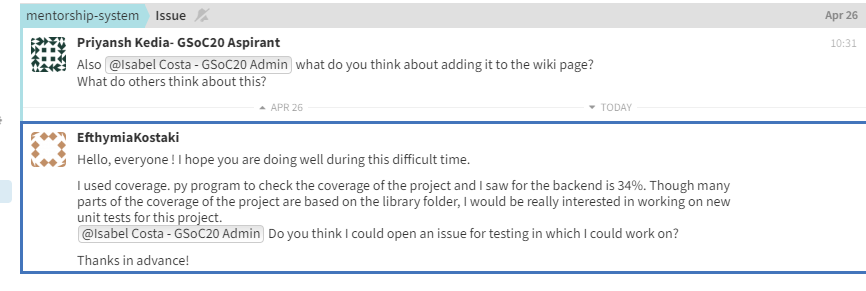
\includegraphics[totalheight=7cm, width=15cm]{testing-coverage.png}}
    \caption{Coverage Discussion}
    \label{fig:verticalcell}
\end{figure}
%-----
\vfill
\clearpage
\hspace{0.5cm}The community agreed that this was a really good idea to focus more on tests in this project and to write new tests or implement changes in the existing ones. They also wanted help into adding the badge of codecoov but since we did not have an account there and it was not our repository we decided that we could not help with that.

What we did find out what-so-ever was that the structure of all the tests was not consistent that's why we proposed this issue:
 
% Image
\begin{figure}[tph!]
\centerline{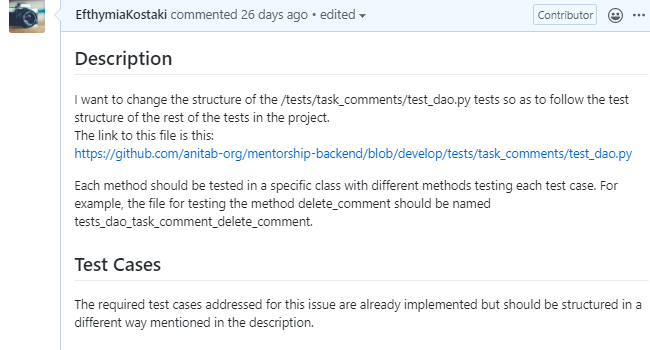
\includegraphics[totalheight=7cm, width=15cm]{issue553.png}}
    \caption{Issue 553}
    \label{fig:verticalcell}
\end{figure}
%-----
\vfill
\clearpage

\subsubsection{Communication with the team}
\hspace{0.5cm}Since the issue was suggested by us we were waiting to hear the response from the main maintainerIsabel about this issue.

The main maintainer Isabel wrote that she believes that there are issues with higher priority but we could go ahead and work on this issue and propose a solution and how we believe it solves the problem. We thought it would be bettor to implement the change and propose the final version of it istead of submitting a Work In Progress Pull Review so the maintainers could check the whole width of our change.
\subsubsection{Our work}
\hspace{0.5cm}We created a specific branch for this issue first locally and then add this branch to our remote repository. We tried to write meaningful messages in our commit messages always following the commit style guide suggested by the project. When we thought that the commit message was not understandable enough we wrote a body in our commit messages and documented further our change.

The problem stemmed from the fact that all the testing of the project was not following the same structure. In some cases the code included in each folder test for base setup and in others not, in others a method was tested in a specific file and in others not, so we thought it was crucial to implement a change which would expand the consistency of the project. We decided that the best strategy for changing the given file was this:
\begin{itemize}
  \item Write a base setup for tests/task\_comments/test\_dao.py
  \item Split  tests/task\_comments/test\_dao.py into four different files. In each one, every method would be tested seperately.
\end{itemize}

To address the first bullet, we needed to understand how a base setup is created and how it is used. We wanted to understand how the setup method is used and how it should be structured to serve our needs. Since, the create\_task\_comment method  was used in all the methods we decided that this was the method which should be used for the setup to avoid code repetition. In order to save each task comment we had to add it in the session of the database and also to commit in the database. In this way, the base setup class which created a new Test Case and all the data, could be used in the unit testing classes we implemented. 

For the second bullet, we splited the test methods into four different files, one for each method:
\begin{itemize}
  \item test\_dao\_create\_task\_comment.py 
  \item test\_dao\_delete\_comment.py  
  \item test\_dao\_modify\_comment.py 
  \item test\_dao\_find\_by\_task\_id.py 
\end{itemize}
\subsubsection{Testing}
\hspace{0.5cm}Testing our addition in this case was harder than in previous points since we were altering the testing of the project. Firstly, we did not delete the class we were altering yet, so we saw the counter of how many tests were already running before our addition. Then, we included our tests and saw if all our tests were passing the testing locally. All the tests were successfully passing in the command line but we wanted to double-check so we run the test\_task\_comments folder seperately through PyCharm. Once we were sure that all our changes were passing we deleted the initial file, commited and created the Pull Request.

\subsubsection{Code Reviews}
\hspace{0.5cm}In the beginning our change received mixed reviews. Of course, there were suggested some minor changes to the code such as to remove unnecessary imports and repetitive code (which turned out to be from the initial testing) but also the argument that this change was not needed right now since there was not a problem.

Regarding the minor changes we addressed them all, since there were important for the crrectness of our change. One suggested change about the repited code turned out to have been from the primary testing so we thought that even though it did not seem so, that it was needed in the project. Turns out it was not so we fixed it.

Regarding the major arguments about the idea of the change and if it was really needed at this point we analyzed our thinking and said that:
\begin{itemize}
\item We started working on this project taking into consideration \textbf{the structure of the tests} in the other parts of the software.
We saw that tasks and mentorship relation folder was structured like the solution we were proposing. 
\item Of course, we saw in some other parts of the project in the testing this structure wasn't followed, but the main idea was the \textbf{consistency} of the testing material so as everyone that needs to write some testing (for example to test a new method) will immediately understand where he/she should do so.
\item \textbf{Expandability of the testing}.
We think this may overlap with the previous point but for example, if we realize at some point that we need on the task comments further testing on the DAO part or if new functionality is added then, according to the other parts of the testing we highlighted in point 1, we shouldn't use the same class for testing the same method more than once and also test the other methods.
\item \textbf{Base test for setup}
We saw that all the methods in task\_comments\_dao were using the same method for the setup that is why we created a test base for the task comments so to avoid code repetition. Our thinking is that the setup test base should be further expanded so the task\_comments\_api classes who test each method use this as well since they all have a setup and some common code. With the change suggested in this pull request, us or someone else interested would be able to intergrade these changes we just mentioned so that the test base covers both the API and the DAO part of the task comments.
\end{itemize}

The maintainer Sanket, who had his doubts about our change after our discussion wrote that he accepts our change and also suggested some change about supporting Python2 in our code. We altered our code and implemented this change but turns out that other parts of the testing still support Python2. We opened another issue for that-namely issue 8. 

\subsubsection{Change}
\hspace{0.5cm}As our change involves the same tests as before we will write in this report only the Test Case we wrote since all the other changes can be found on Github. This file is included in: tests/task\_comments/task\_comments\_base\_setup.py

% Image
\begin{figure}[tph!]
\centerline{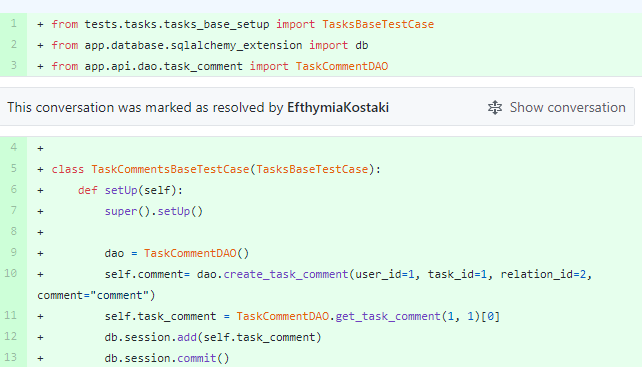
\includegraphics[totalheight=7cm, width=15cm]{issue553-change.png}}
    \caption{Issue 553 Change}
    \label{fig:verticalcell}
\end{figure}
%-----
\vfill
\clearpage

\subsection{Issue 7 - Fix description messages on Backend Server - \emph{Pending}  \#577}
Similar to Issue 2 but addressed the whole project namely the resources Admins and Users.
\subsubsection{Issue}
% Image
\begin{figure}[tph!]
\centerline{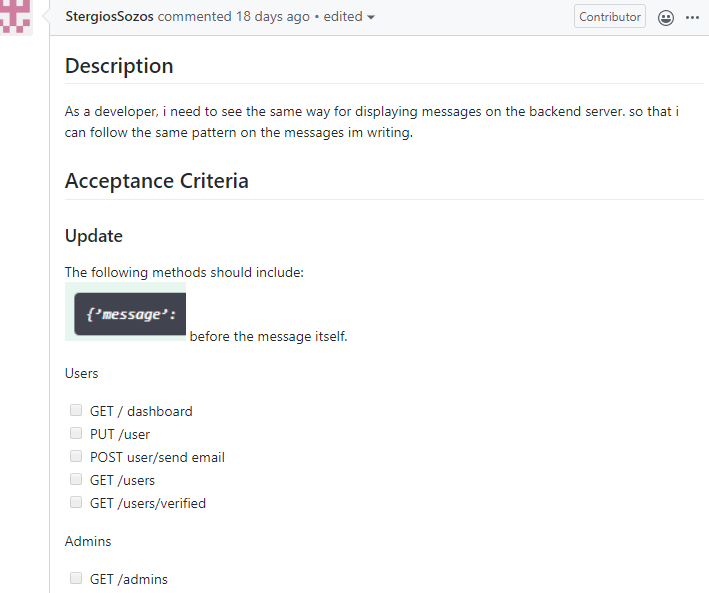
\includegraphics[totalheight=10cm, width=15cm]{issue577.png}}
    \caption{Issue 577}
    \label{fig:verticalcell}
\end{figure}
%-----
\vfill
\clearpage

\subsubsection{Communication with the team}
Since we were the ones who created the issue we did not want to start working in it before we were assigned. We asked siddhipandare if we could be assigned to this  issue and said that yes we could start working on it.

\subsubsection{Documentation}
This change required a change in the documentation of the resources. This was labeled in the issue as a label by the maintainers. 

\subsubsection{Our work}
Since, we were already familiar in the way this issue should be solved we utilized the knowledge from issue 2 to correct the messages in the resources of Users and Admins, change to fstrings and create new specific messages in the messages.py. For more specifics on how we worked on that issue refer to issue 2.

\subsubsection{Testing}
\begin{itemize}
  \item While running the local server and checking the UI the changes are visible.
  \item All Travis CI tests have passed
\end{itemize}

\subsubsection{Code Reviews}
Unfortunately, this review has not received a code review yet probably because of the limit of the bandwidth of the maintainers.

\subsubsection{Change}
We changed three files so we present here only our changed code. 

\begin{itemize}
  \item app/api/resources/admin.py 
\lstset{language=Python}
\begin{lstlisting}
@admin_ns.response(HTTPStatus.OK, 
    f"{messages.GENERAL_SUCCESS_MESSAGE}",
    public_admin_user_api_model)
   @admin_ns.doc(	  
     responses={	    
        HTTPStatus.UNAUTHORIZED: f"{messages.TOKEN_HAS_EXPIRED}<br>"
        f"{messages.TOKEN_IS_INVALID}<br>"	    
        f"{messages.AUTHORISATION_TOKEN_IS_MISSING}"
        }	        
    )	    
\end{lstlisting}
 \item app/api/resources/user.py
\lstset{language=Python}
\begin{lstlisting}
@users_ns.doc(
  responses={	  
      HTTPStatus.UNAUTHORIZED:
      f"{messages.TOKEN_HAS_EXPIRED}<br>"	       
      f"{messages.TOKEN_IS_INVALID}<br>"	      
      f"{messages.AUTHORISATION_TOKEN_IS_MISSING}"	           
      }	        
    )	    

@users_ns.response(HTTPStatus.CREATED, 
        f"{messages.GENERAL_SUCCESS_MESSAGE}"
        , public_user_api_model)

@users_ns.response(HTTPStatus.BAD_REQUEST, 
    f"{messages.INVALID_INPUT}")

@users_ns.doc(
    responses={
    HTTPStatus.UNAUTHORIZED: 
    f"{messages.TOKEN_HAS_EXPIRED}<br>"
    f"{messages.TOKEN_IS_INVALID}<br>" 
    f"{messages.AUTHORISATION_TOKEN_IS_MISSING}"
    }
)

@users_ns.response(HTTPStatus.OK, 
         f"{messages.EMAIL_VERIFICATION_MESSAGE}")
@users_ns.response(HTTPStatus.BAD_REQUEST, 
         f"{messages.INVALID_INPUT}")
@users_ns.response(HTTPStatus.FORBIDDEN, 
         f"{messages.USER_ALREADY_CONFIRMED_ACCOUNT}")
@users_ns.response(HTTPStatus.NOT_FOUND,
         f"{messages.USER_DOES_NOT_EXIST}")

@users_ns.response(HTTPStatus.OK, f"{messages.SUCCESSFUL_REFRESH}",
         refresh_response_body_model)

@users_ns.response(HTTPStatus.OK, f"{messages.SUCCESSFUL_LOGIN}",
         login_response_body_model)

@users_ns.response(HTTPStatus.OK, f"{messages.SUCCESSFUL_RESPONSE}",
         home_response_body_model)

@users_ns.response(HTTPStatus.OK, f"{messages.GENERAL_SUCCESS_MESSAGE}", 
         dashboard_response_body_model)

@users_ns.response(HTTPStatus.NOT_FOUND,
         f"{messages.USER_NOT_FOUND}")
\end{lstlisting}
 \item app/messages.py
\lstset{language=Python}
\begin{lstlisting}
INVALID_INPUT = {"message": "Invalid input."}
GENERAL_SUCCESS_MESSAGE = {
    "message": "Success."
}

SUCCESSFUL_REFRESH = {
    "message": "Successful refresh."
}

SUCCESSFUL_RESPONSE = {
    "message": "Successful response."
}

SUCCESSFUL_LOGIN = {
    "message": "Successful login"
}
\end{lstlisting}
\end{itemize}

\section{Our Legacy}
\subsection{Issue - Add only Python3 support in tests \#595}
% Image
\begin{figure}[tph!]
\centerline{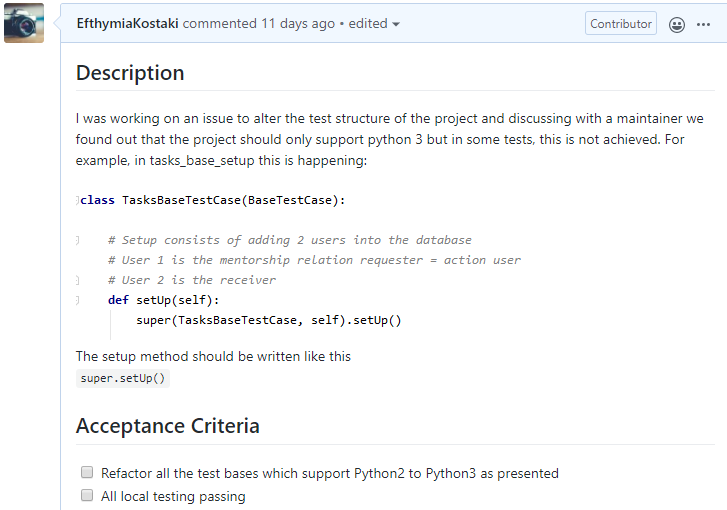
\includegraphics[totalheight=10cm, width=15cm]{issue595.png}}
    \caption{Issue 595}
    \label{fig:verticalcell}
\end{figure}
%-----
\vfill
\clearpage
\section{Conclusion}
Contributing to an open-source project
 enriched our understanding  of program 
development and urged us to try to establish 
possible improvements. We were able to express
 our opinion with facts and use the terminology we
 learned during the course. We researched a lot with
 or without the guidance of the open-source community
 and offered feasible solutions. In the future, we want
 to continue contributing to other open-source projects.
\section*{References}
[1] https://github.com/anitab-org
\newline
[2] https://github.com/anitab-org/mentorship-android
\newline
[3] https://github.com/anitab-org/mentorship-backend
\end{document}